In this chapter we will look at \textbf{Large Multimodal Models} (LMMs). No, \textit{you heard me right}, we will not be looking at \textbf{Large Language Models} (LLMs), in which the data modality is primarily textual, but at Large Multimodal Models, which can handle multiple types of input data, including text, images, audio, video, and sometimes other types of data such as sensory data.

We will look at \textbf{multimodal architectures}, which are computational models designed to process and integrate data from different modalities or input types. To get to LMMs, we will look at \textbf{Large Vision-Language Models}, focusing on the \textit{Image Encoder} in a multimodal setup. Using this setup, we aim to create networks capable of consuming different types of input to learn more robust visual representations.

\begin{figure}[!htbp]
    \centering
    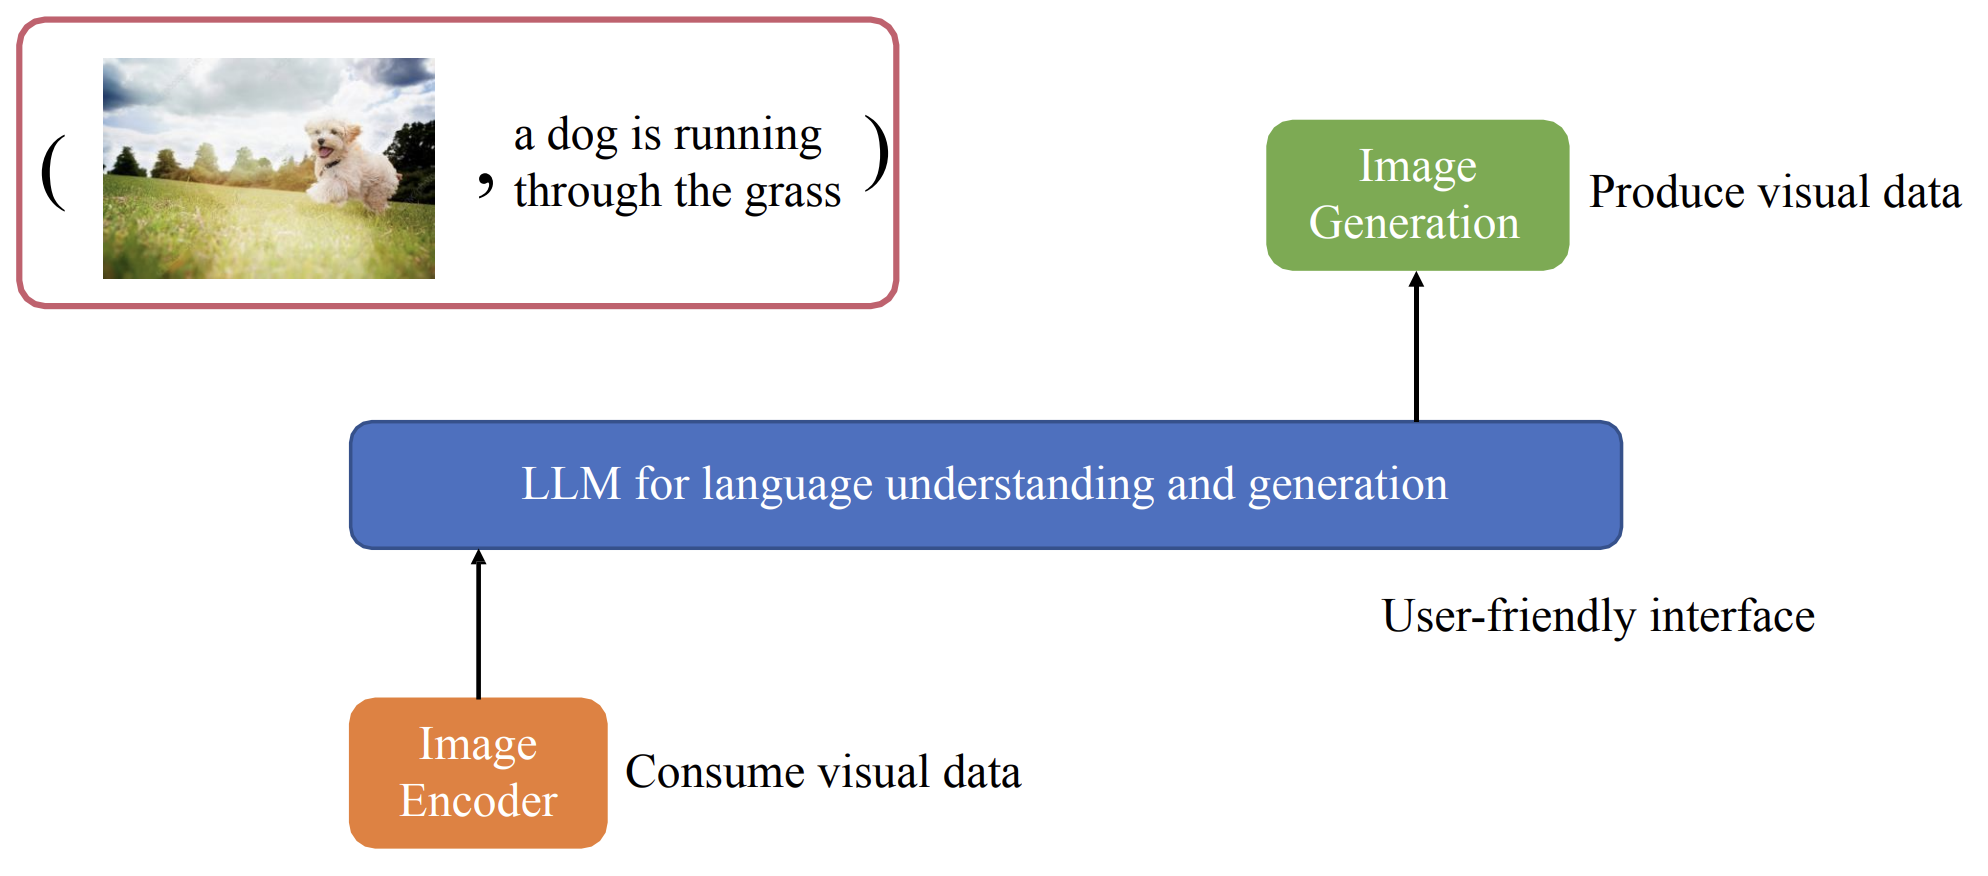
\includegraphics[width=0.75\linewidth]{tikz/chapter11 - Large Vision-Language Models.png}
    \caption{{\color{red}\colorbox{pink}{Tikz TO-DO}} Large Vision-Language Models Idea}
\end{figure}

As you can see, the goal is to create an encoder that learns a representation of our data (pairs of images and text), and then use an LLM as a frontend for generation.

Currently, all methods for training an encoder share the same goal: to \textbf{build a robust model capable of learning robust representations of data}. Let us now look at the four main methods of training an encoder:

\begin{itemize}
    \item \textbf{Supervised Learning}: This is the first approach we used to train encoders, in which models are trained using large amounts of manually annotated data. Although this method can produce excellent results, it has a significant bottleneck due to the high cost and time required for human annotation.
    
    \item \textbf{Image-Only (Non-) Contrastive Learning}: This approach exploits methods such as the DINO (DIstillation with NO labels) model, which allows encoders to be trained using images only, without the need for labels. Through contrastive learning techniques, the model learns to distinguish between similar and different representations.
    
    \item \textbf{Masked Image Modeling}: Inspired by the invention of the BERT model for language, this method applies a similar concept to images. Some parts of the image are "masked" and the model's task is to predict the missing parts. This process forces the encoder to understand the visual context and develop a robust internal representation.
    
    \item \textbf{Contrastive Language-Image Pre-Training}: Using the CLIP (Contrastive Language-Image Pre-Training) model developed by OpenAI and its variants, this approach involves training an encoder that can understand both language and images. The model is trained to correlate images and corresponding text descriptions, allowing it to create visual representations that are semantically aligned with the text. This method has shown outstanding results in a variety of multimodal tasks and has opened up new possibilities for the integration of different data modalities.
\end{itemize}

In the next sections, we will examine these approaches in detail.

\section{Image-Only (Non-) Contrastive Learning}

\subsection{SimCLR}

The first alternative to the previous class of models that emerged was \textbf{SimCLR}, introduced in the article \href{https://arxiv.org/pdf/2002.05709}{"A Simple Framework for Contrastive Learning of Visual Representations" (Chen et al.)}.

\begin{figure}[!htbp]
    \centering
    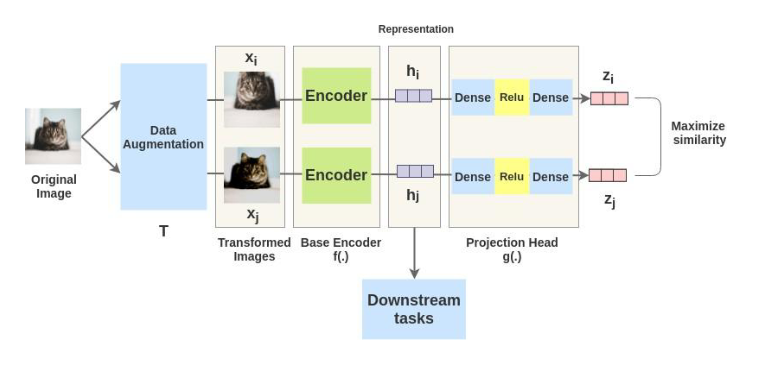
\includegraphics[width=0.75\linewidth]{tikz/chapter11 - SimCLR.png}
    \caption{{\color{red}\colorbox{pink}{Tikz TO-DO}} SimCLR architecture}
\end{figure}

Here's how it works: given an image, \textbf{two different data augmentations} are applied. Each augmented image is then processed by an encoder, producing corresponding fixed latent representation vectors. These vectors are subsequently passed through a \textbf{projection head}, which maps them to another latent space, resulting in the vectors $z_i$ and $z_j$.

Each module of the projection head consists of a sequence of fully connected layers, ReLU activations and a final dense layer. The vectors $z_i$ and $z_j$ are used in the \textbf{contrast loss function}, specifically \textbf{InfoNCE}, to perform training. The goal is to maximize the agreement between augmentations by determining whether they come from the same image or not.

This approach is \textbf{contrastive} because we impose two constraints on the model parameter space: \textbf{positive examples will have similar representations while negative examples will have very dissimilar representations}.

In this case, \textbf{projection head is discarded for downstream tasks}, since the best representations are $h_i$ and $h_j$ instead of $z_i$ and $z_j$. However, this model requires a large batch size to ensure a sufficient number of negative samples for each class.

Recent research has addressed this problem using the principle that the representations of a sample and its transformation should be similar. Alternatives include \textbf{DINO}, which uses a method based on \textbf{clustering}.

\subsection{DINO}

The article \href{https://arxiv.org/pdf/2104.14294}{"Emerging Properties in Self-Supervised Vision Transformers" (Caron et al.)} introduces DINO (Distillation with No Labels), which is a Vision Transformer model that employs self-supervised loss. It is widely recognized for its ability to compute segmentation maps that emerge from the transformer's self-attention modules.

The architecture uses a \textbf{teacher-student} framework with a \textbf{cross-entropy loss}. The student network extracts the parameters of interest, and since DINO is part of the clustering approach, the output of the student network goes through a softmax function to determine whether an image belongs to a certain cluster.

This produces a probability distribution, allowing training with a \textbf{self-supervised cross-entropy loss}. The teacher network is updated using the \textbf{exponential moving average (EMA)} of the parameters learned from the student network.

To ensure that the teacher makes accurate predictions for a given class, centering and softmax layers are added. The centering layer subtracts the average feature and the output is refined using a low temperature softmax.

The gradient is propagated only through the student network, allowing centering to be used on the teacher model.

\begin{figure}[!htbp]
    \centering
    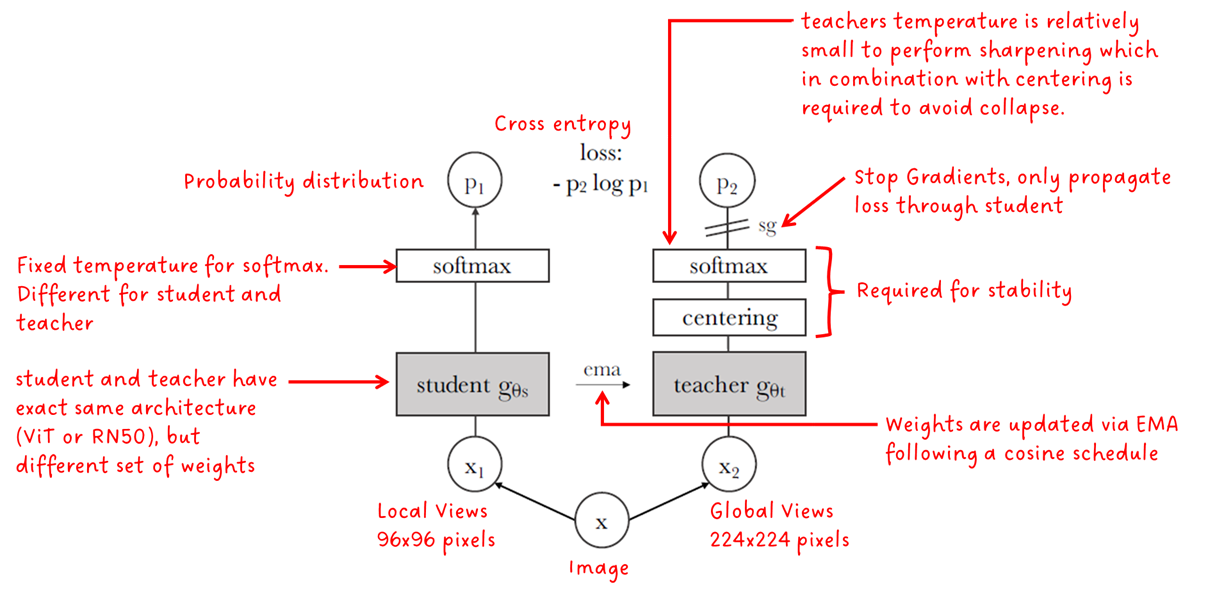
\includegraphics[width=0.75\linewidth]{tikz/chapter11 - DINO.png}
    \caption{{\color{red}\colorbox{pink}{Tikz TO-DO}} DINO Architecture}
\end{figure}

Thus, clustering tends to solve the batch size problem of SimCLR \textbf{learning a powerful visual encoder through self-supervised loss}.


\section{Masked Image Modeling}

In this learning class, models are trained to predict a missing part of the input (masked) given the other (unmasked) information.

\subsection{BEiT}

Following the BERT model developed in the area of natural language processing, Microsoft proposed a masked image modeling task to pre-train Vision Transformers in the article \href{https://arxiv.org/pdf/2106.08254}{"BEiT: BERT Pre-Training of Image Transformers" (Dong et al.)}.

The model works by taking an image and dividing it into patches. Next, \textbf{some of these patches are masked and all patches are flattened into a vector}. This vector becomes the input (plus positional embedding) of the \textbf{encoder BEiT}, which is pre-trained similarly to the BERT model in natural language processing. Only embeddings related to the masked tokens are then retrieved. The chosen embeddings are then passed as input to an additional encoder, the \textbf{Masked Image Modelling Head}. This represents what we ultimately want to learn. To do this, we employ supervised help.

To facilitate this process, an additional network is used. Before pre-training, an "image tokenizer" is learned through VQ-VAEs or GANs, which \textbf{tokenizes an image into discrete visual tokens, which act as supervisors for the encoder}. The Masked Image Modelling Head can thus be seen as a form of \textbf{knowledge distillation} (Process in which a smaller model, the "student", learns to replicate the behavior of a larger, more complex model, the "teacher") between the image tokenizer and the BEiT encoder, with the key difference being that the BEiT encoder sees only part of the image.

In the end, we use a pre-trained decoder to predict the masked visual tokens.

\begin{figure}[!htbp]
    \centering
    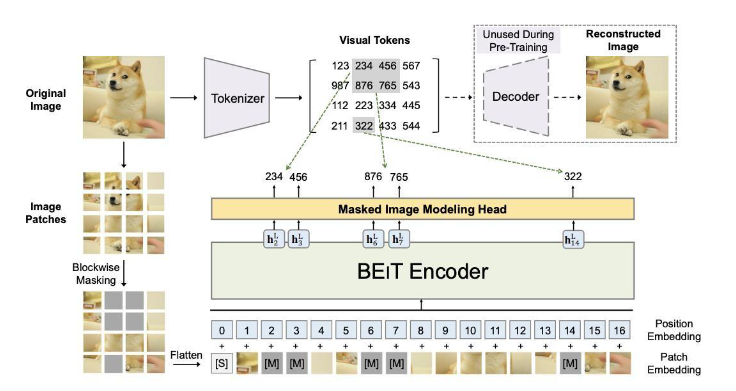
\includegraphics[width=\linewidth]{tikz/chapter11 - BEiT.png}
    \caption{{\color{red}\colorbox{pink}{Tikz TO-DO}} BEiT Architecture}
\end{figure}

The model works rather well with fine-tuning rather than pre-training. Of course, one reason related to this fact is the complexity of the model. As a result, variants have been developed.

\subsection{MAE}

\textbf{MAE} is a variant of BEiT introduced by Meta in the article \href{https://arxiv.org/pdf/2111.06377}{"Masked Autoencoders Are Scalable Vision Learners" (He et al.)}. It uses \textbf{pixel values as targets} instead of visual tokens. The model can be very aggressive in masking patches, since a large random subset of the images (for example 75\%) can be masked. Thus, the encoder is trained to \textbf{produce representations of only the visible patches}. Before the decoder, masked patches are remapped with latent representations, and then the decoder reconstructs the original image.

\begin{figure}[!htbp]
    \centering
    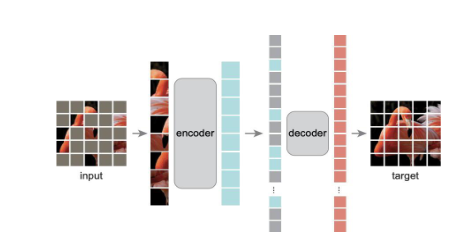
\includegraphics[width=\linewidth]{tikz/chapter11 - MAE.png}
    \caption{{\color{red}\colorbox{pink}{Tikz TO-DO}} MAE Architecture}
\end{figure}


\section{Contrastive Language-image Pre-training}

\textit{We have come to the most fascinating and juicy part of this chapter.} These types of models represent the current state of the art. 

\subsection{CLIP}

Introduced in \href{https://arxiv.org/pdf/2103.00020}{"Learning Transferable Visual Models From Natural Language Supervision" (Kim et al.)}, CLIP is a multimodal model developed by OpenAI, designed to integrate and understand both textual and visual information. CLIP represents a significant breakthrough in the field of multimodal models because of its ability to correlate images and text in a highly efficient and scalable manner.

CLIP combines two main neural networks:
\begin{itemize}
    \item \textbf{The Image Encoder}: It uses a Vision Transformer based network or deep convolutional network to convert images into embedding vectors.
    \item \textbf{The Text Encoder}: Employs a Transformer-type neural network, similar to that used in language models such as GPT, to convert texts into embedding vectors.
\end{itemize}

The main goal of CLIP is to create a \textbf{shared embedding space in which images and text descriptions are semantically aligned}. During training, the model uses a \textbf{contrastive learning} technique to optimize the similarity between image embeddings and corresponding text descriptions, while minimizing the similarity between images and unrelated text. This approach allows CLIP to make inferences and classifications based on text descriptions, without the need to train task-specific models.

CLIP was trained on a large and diverse dataset containing approximately \textbf{400 million image-text pairs taken from the Internet}. Although this dataset is sizable, even larger datasets, such as LAION, containing billions of images, are now also being used.

\begin{figure}[!htbp]
    \centering
    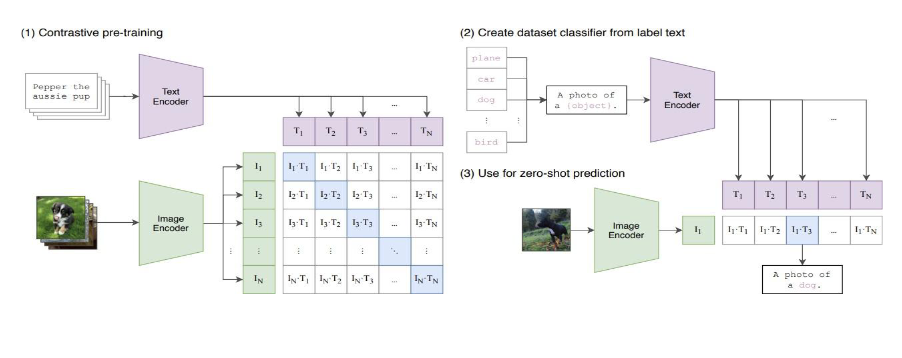
\includegraphics[width=\linewidth]{tikz/chapter11 - CLIP.png}
    \caption{{\color{red}\colorbox{pink}{Tikz TO-DO}} CLIP Architecture}
\end{figure}

In essence, CLIP aims to maximize the similarity between pairs of images and texts, corresponding to \textbf{\textcolor{mybluee}{the diagonal of the similarity matrix}} you see in the figure. At the same time, it tries to minimize the similarity (increase dissimilarity) between all other pairs, that is, between unrelated images and texts. 

CLIP's capabilities extend to numerous applications, called \textbf{downstream tasks}, such as image classification and search: it can be used to search for images based on text descriptions and vice versa. A notable aspect of CLIP is its \textbf{zero-shot learning} capability, which allows it to generalize to new categories without the need for additional training specific to those categories. 

However, CLIP has some limitations:
\begin{enumerate}
    \item \textbf{Limited Capability}: CLIP is limited to connecting image and text embedding spaces.
    \item \textbf{Use Restricted to Specific Tasks}: Although it excels at classification and searching, CLIP is less suitable for more complex tasks such as text generation or visual question answering.
    \item \textbf{Language Generation Capability Absence}: CLIP lacks the ability to generate language, making it less suitable for open-ended tasks such as caption generation or visual question answering.
\end{enumerate}

\textit{So, how can we improve the model?} We can make improvements in three main areas: \textbf{Data Scalability}, \textbf{Model Design} (for both image and text encoder) and \textbf{Objective Functions} (contrastive learning).

In the next subsections we will explore in detail the various improvements proposed for CLIP and see some models that implement these ideas.


\subsection{Data Scaling Improvement}

 This paper used pre-trained open CLIP with LAION-2B across various scales, namely model, data, ecc..
The take home message is that scale matter.

\href{https://arxiv.org/pdf/2212.07143}{"Reproducible scaling laws for contrastive language-image learning" (Jitsev et al.)} studied the use of pre-trained CLIP with the LAION-2B dataset at different scales, including models and data. The main message is that \textbf{scale of dataset is crucial}.

\textit{But how can we scale further?} One possible solution is to search for next-generation image-text datasets. However, in \href{https://arxiv.org/pdf/2304.14108}{"DataComp: In search of the next generation of multimodal datasets" (Ilharco et al.)}, researchers found that \textbf{filtering the data} provided to the model leads to better results even with smaller datasets.


\subsection{Image Model Design Improvement: FLIP}



A Model Design Improvement for the image encoder is \textbf{FLIP}, introduced in , which tried to scale CLIP training (more efficient) via randomly masking out image patches with a high masking ratio. This allows the image encoder to process just the non-masked patches. Thus, during training we still use CLIP loss, but no reconstruction of masked patches is made.

A significant improvement in model design for the image encoder is FLIP, introduced in \href{https://arxiv.org/pdf/2212.00794}{"Scaling Language-Image Pre-training via Masking" (Li et al.)}. This approach aims to make CLIP training more efficient by \textbf{randomly masking image patches with a high masking ratio}. This allows the image encoder to process only the unmasked patches. During training, CLIP loss is still used, but no reconstruction of masked patches is performed.

Results have shown that this approach not only does not compromise performance, but \textbf{also improves training efficiency}.

\begin{figure}[!htbp]
    \centering
    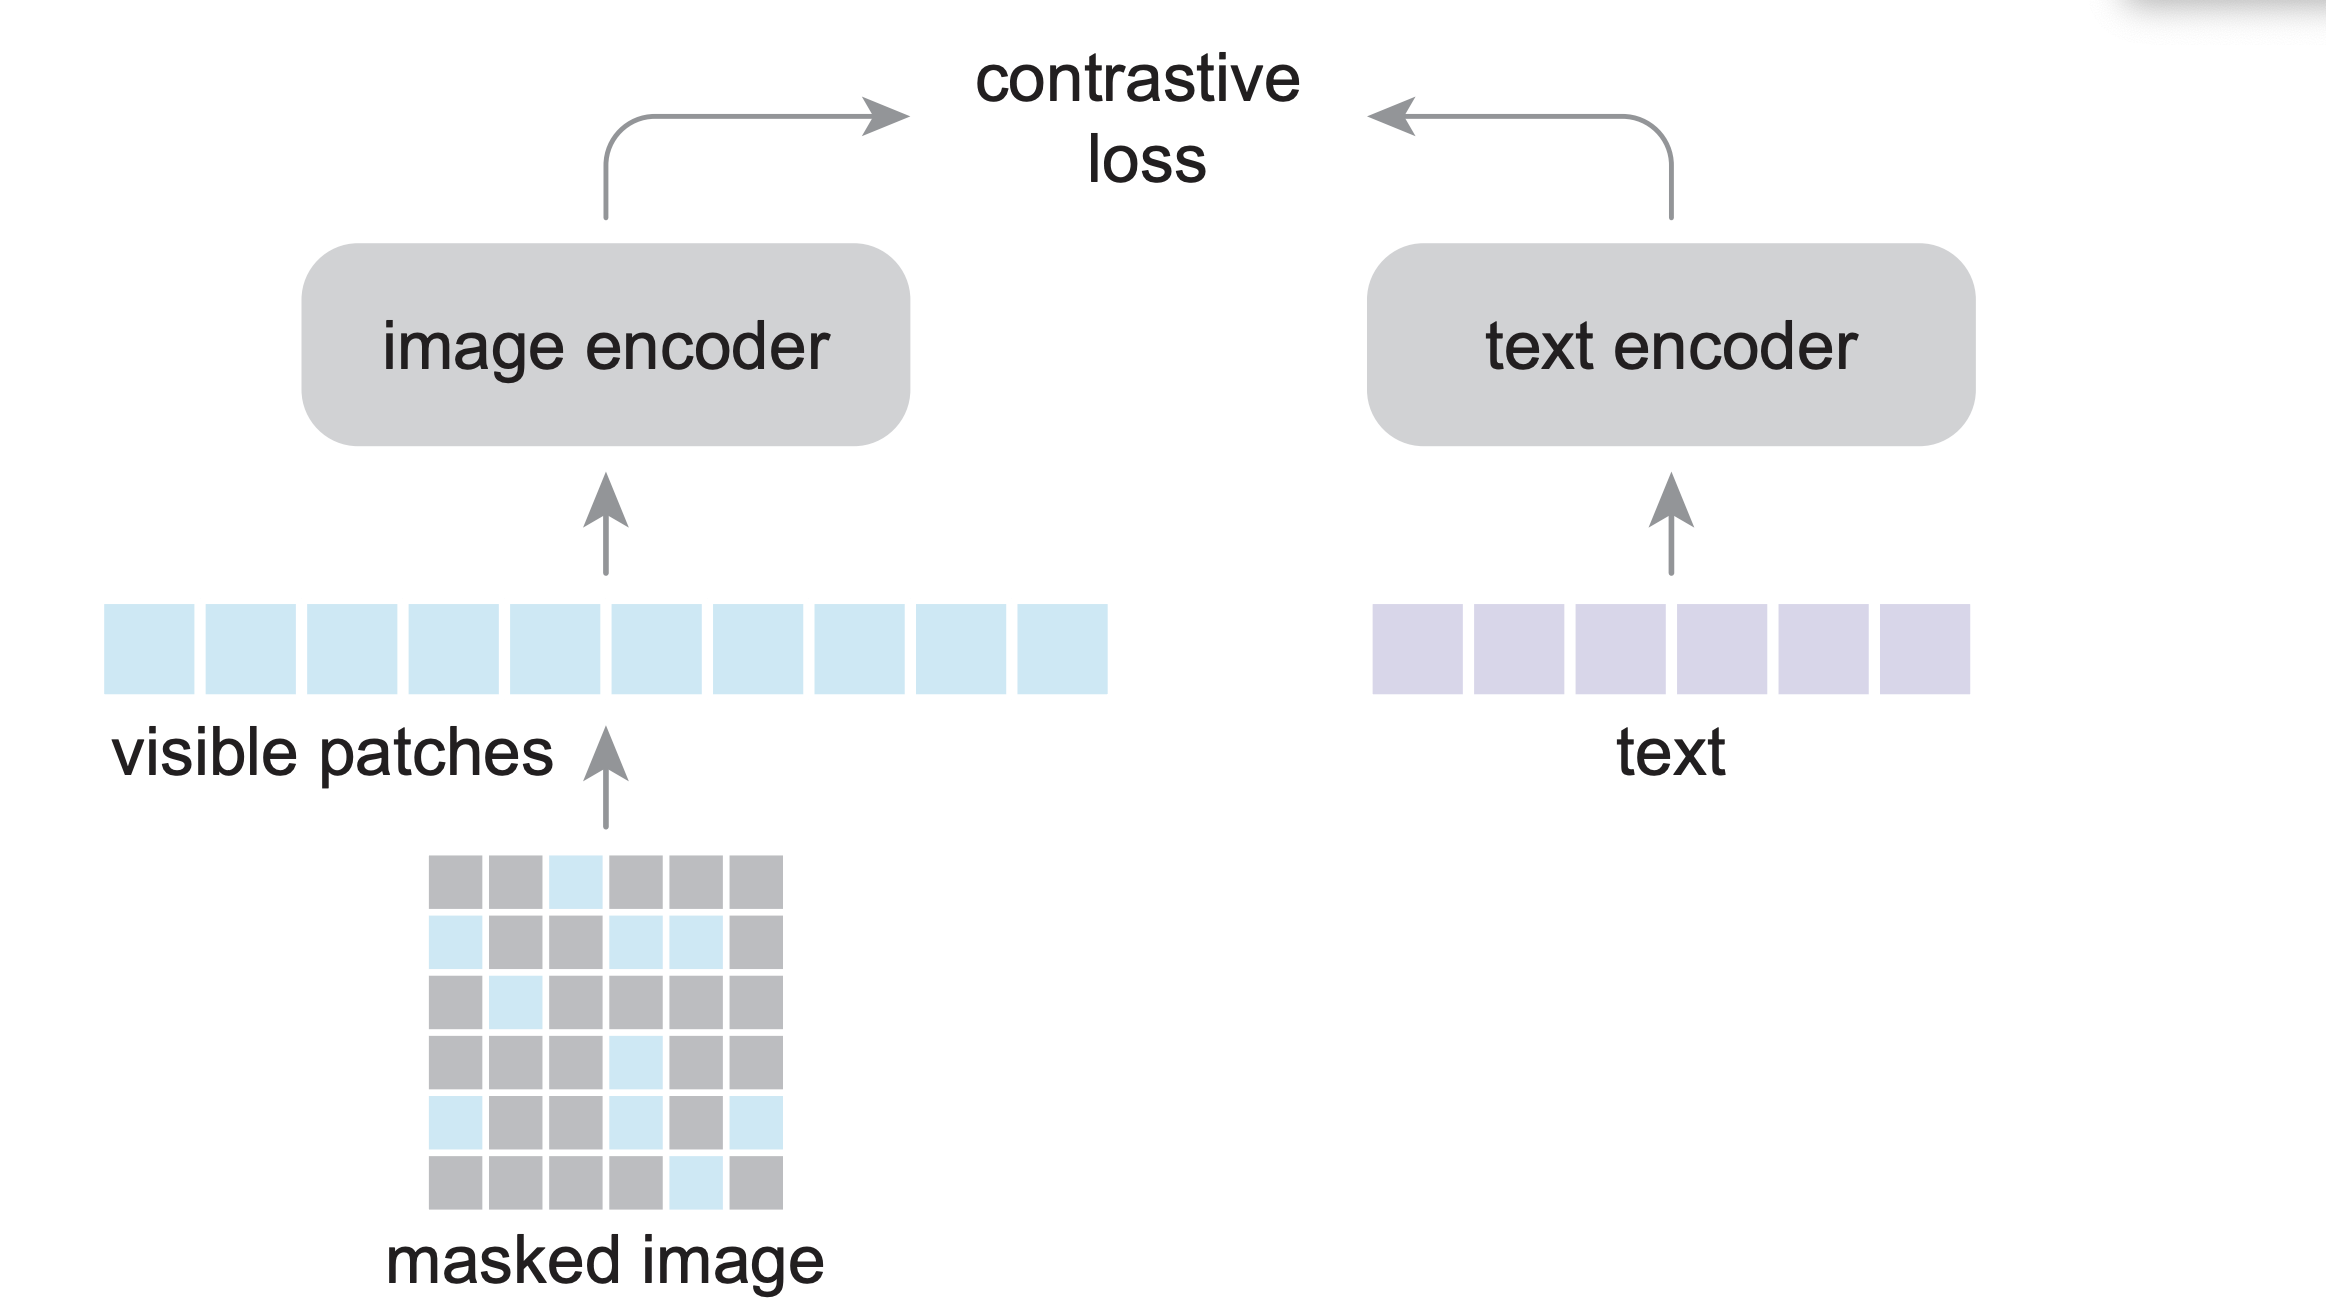
\includegraphics[width=0.8\linewidth]{tikz/chapter11 - FLIP.png}
    \caption{{\color{red}\colorbox{pink}{Tikz TO-DO: only the left}} FLIP Architecture}
\end{figure}

\subsection{Language Model Design Improvement: K-LITE}

Because classes are very specific, the work \href{https://arxiv.org/pdf/2204.09222}{"K-LITE: Learning Transferable Visual Models with External Knowledge" (Shen et al.)} introduces a mechanism to extend text knowledge via \textbf{external knowledge} in order to provide more detailed information. For example, WordNet or Wikipedia can be used. This is easily accomplished since the text encoder can be fed with input of arbitrary length (original text + external knowledge).

The mechanism of knowledge expansion takes place in two stages: during training, the \textbf{model acquires the ability to read and understand a specific knowledge source}. During evaluation, the knowledge provides an \textbf{additional source of information to improve model inference}.

Results showed that f\textbf{or datasets containing specific images}, such as the Flowers dataset, \textbf{knowledge expansion led to improvements in performance}, as the additional knowledge helped to better discriminate between classes. However, for datasets such as Eurosat, the approach performed poorly because the additional knowledge retrieved was irrelevant to the image. 


\subsection{Model Design Improvement: Multi Modalities}

In this case, improvement is achieved by adding more modes than just the traditional two (such as audio, video, etc.). For example, in the study \href{https://arxiv.org/pdf/2305.05665}{"ImageBind: One Embedding Space To Bind Them All" (Girdhar et al.)}, Meta introduced ImageBind, a model that uses one of the seven available modes as an anchor (images) and aligns the other modes to this key mode. In this way, all modes are \textbf{linked to a common space}. A pre-trained CLIP is used and kept frozen, i.e., only the encoders for the other modes are learned to align the CLIP embedding space.

\begin{figure}[!htbp]
    \centering
    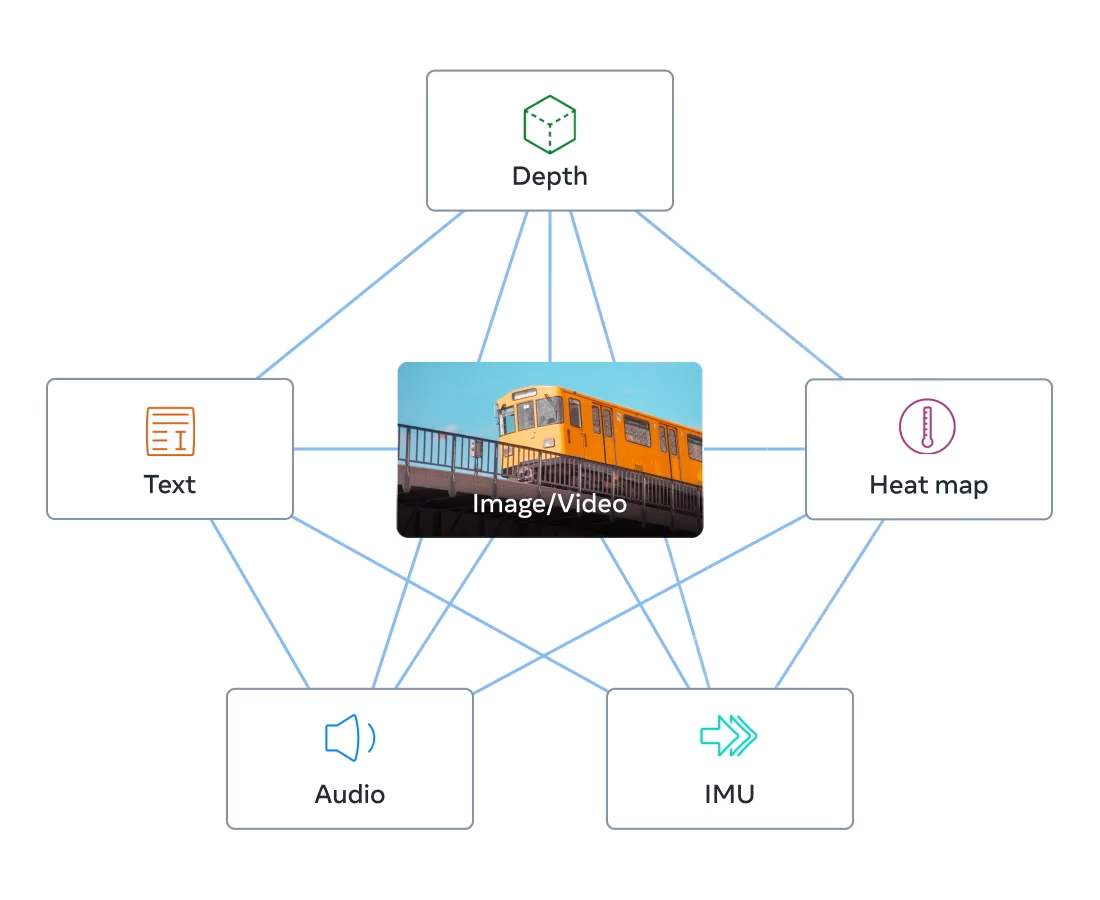
\includegraphics[width=0.6\linewidth]{tikz/chapter11 - ImageBind.png}
    \caption{{\color{red}\colorbox{pink}{Tikz TO-DO}} ImageBind Idea of Shared Embedding Space}
\end{figure}

The model employs pairs of modalities (I,M), where I signifies images and M is another modality, to learn a \textbf{single joint embedding}. Each modality’s embedding is aligned with image embeddings, for instance, text is aligned with images using web data. The embeddings and encoders are optimized using an \textbf{InfoNCE loss}.

The model uses mode pairs \((I, M)\), where \(I\) represents images and \(M\) is another mode, to learn a \textbf{unique joint embedding}, indeed every embedding is aligned with image embeddings. The embeddings and encoders are optimized using a \textbf{InfoNCE (Information Noise-contrastive Estimation) loss}.

ImageBind showed an \textbf{emergent behavior}: the model is able to align two different modes \((M_1, M_2)\) even though it was trained only with pairs \((I, M_1)\) and \((I, M_2)\). For example, it obtains state-of-the-art results in zero-shot text-audio classification without having been exposed to paired audio-text samples. Hence, given an audio of the sound of a fire, the model can generate an image or video of the fire.


\subsection{Model Design Improvement: STAIR}
One of the limitations of CLIP is the lack of interpretability in the image embedding space. However, thanks to \href{https://arxiv.org/pdf/2301.13081}{"STAIR: Learning Sparse Text and Image Representation in Grounded Tokens" (Zhang et al.)}, it is possible to achieve better performance than CLIP with a significant improvement in interpretability. Instead of using dense, uninterpretable representations, STAIR creates a \textbf{sparse, semantic representation of images and texts}. 

STAIR is \textbf{based on a large vocabulary of words and phrases}, known as a "dictionary of tokens". Each word in the dictionary is considered a unique token, representing a specific concept or term.

For each image or text, STAIR constructs an embedding space in which \textbf{each dimension of the vector corresponds to a vocabulary word}. In other words, images and texts are represented as vectors scattered throughout this space, reflecting which and how many tokens are present and relevant.

Each token in the dictionary is \textbf{associated with a non-negative scalar value}, indicating the token's importance to the image or text in question.  Finally, STAIR uses a unit called the \textbf{Token Projection Head} to project representations into its sparse embedding space.

Thanks to this method, we can observe the relevance of each word in the embedding space. In the figure below, we consider the first 20 tokens predicted by STAIR for an image and represent them graphically with a font size indicating the prediction weight.

\begin{figure}[!htbp]
    \centering
    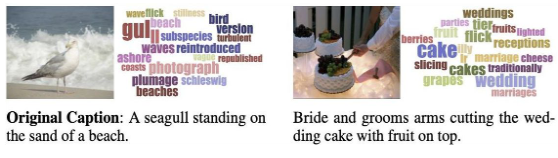
\includegraphics[width=0.8\linewidth]{tikz/chapter11 - STAIR Results.png}
    \caption{{\color{red}\colorbox{pink}{Tikz TO-DO}} STAIR Results}
\end{figure}



\subsection{Objective Functions Improvement: FILIP}

As we have stated, another way of improving clip is to improve the objective function and FILIP, introduced in \href{https://arxiv.org/pdf/2111.07783}{"FILIP: Fine-grained Interactive Language-Image Pre-Training" (Yao et al.)}, belongs to this category. 

FILIP uses two main encoders:
\begin{itemize}
    \item \textbf{Visual Encoder}: Based on Vision Transformer (ViT), this encoder takes as input images divided into patches. A special token \texttt{[CLS]}, representing the image as a whole, is added to these patches. The patches and the \texttt{[CLS]} token are linearly projected and then processed by the model.
    \item \textbf{Text Encoder}: After embedding the words, the text is processed by a Transformer-only decoder. This model handles the token sequences generated by the words in the text.
\end{itemize}


The objective function of FILIP is fine-grained alignment:
\begin{itemize}
    \item \textbf{Token-wise similarity}: FILIP calculates the \textbf{similarity between each token in the text and each patch in the image}. This process allows you to see how each word in the text aligns with different parts of the image.
    \item \textbf{Pooling and Aggregation}: After calculating the similarity matrix between tokens and patches, FILIP uses max pooling to \textbf{aggregate these similarities}, making the representations more useful for later tasks.
\end{itemize}

FILIP is designed to learn detailed alignment between words and image patches, improving visual and textual understanding. The image below shows an example with the class label "balloon" (in this case class 5), which is entered into the prompt "\texttt{[BOS]} a photo of a balloon. \texttt{[EOS]}" and tokenized into a sequence of 8 tokens. \textbf{The model learns the corresponding tokens that are activated in the patches of the image where the class is visible.} 

\begin{figure}[!htbp]
    \centering
    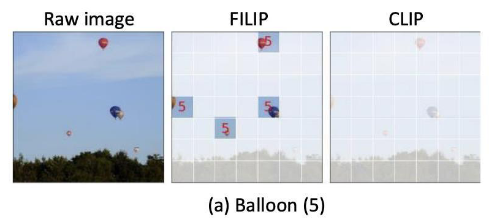
\includegraphics[width=0.8\linewidth]{tikz/chapter11 - FILIP vs CLIP.png}
    \caption{{\color{red}\colorbox{pink}{Tikz TO-DO}} An example of word-patch visualization with FILIP}
\end{figure}


\subsection{Objective Functions Improvement: CoCa}

The CoCa model, introduced in the paper by Google \href{https://arxiv.org/pdf/2205.01917}{"CoCa: Contrastive Captioners are Image-Text Foundation Models" (Yu et al.)}, represents a significant advance in the integration of contrastive learning with language generation. CoCa enhances CLIP by adding a \textbf{generative branch} (Captioner), thus allowing the model to perform an additional task: captioning images. This approach led to the creation of a \textbf{basic encoder-decoder image-text pretrained model}, jointly trained using a contrastive loss and a captioning loss. As a result, the model is not only limited to visual recognition tasks, but is also capable of performing downstream tasks, as you can see from the figure below.

\begin{figure}[!htbp]
    \centering
    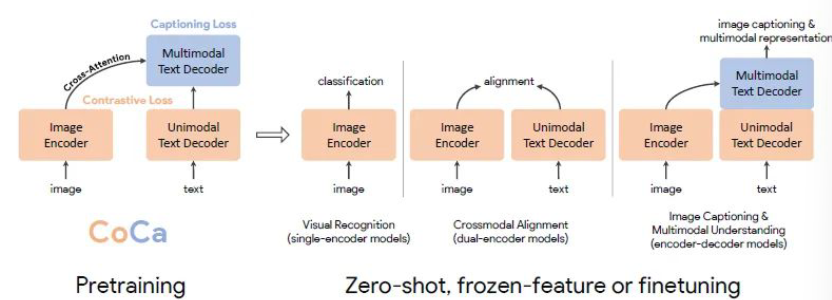
\includegraphics[width=\linewidth]{tikz/chapter11 - CoCa.png}
    \caption{{\color{red}\colorbox{pink}{Tikz TO-DO}} CoCa}
\end{figure}

\textbf{CoCa unifies three paradigms into one model}: single-encoder, dual-encoder and encoder-decoder. The model has several key features. Cross-attention is omitted in the unimodal decoder layer, thus allowing only textual representations to be encoded. The multimodal decoder, on the other hand, uses cross-attention on the image encoder outputs to learn multimodal representations. While the dual-encoder approach encodes text as a whole, the generative approach aims for detailed granularity. This means that the model \textbf{not only creates a global representation of the text, but also predicts word by word the text associated with the image}.

This is done \textbf{autoregressively}, using this formula: $L_\text{Cap} = - \sum_{t=1}^{T}\log P_{\theta}(y_t|y_{<t},x) $

This loss reflects one of the typical ways to generate a text $y$ using the probability of generating a token $y_t$ given all previous predictions $y_{<t}$ and visual information $x$ from the image encoder. The training approach is termed \textbf{autoregressive learning}, and the loss maximizes the conditional probability ($P_\theta$) of paired text images under forward autoregressive factorization.

\subsection{Objective Functions Improvement: SimVLM}


In \href{https://arxiv.org/pdf/2108.10904}{"SimVLM: Simple Visual Language Model Pretraining with Weak Supervision" (Wang et al.)}, SimVLM is introduced as a \textbf{precursor to CoCa} by the same authors. Although SimVLM was an innovative attempt, it wasn't as competitive as CLIP.

The architecture of SimVLM employs a transformer encoder-decoder model. The idea is to have the model generating text sequentially, using the preceding tokens and visual context to predict each subsequent token.

Ultimately, what we have seen so far are three different design approaches for tackling Vision-Language models:
\begin{itemize}
    \item \textbf{Dual Encoders} (CLIP): Text cannot be generated, but it excels in matching images and texts.
    \item \textbf{Encoder-Decoder} (SimVLM): Text can be generated, but it doesn't compete as effectively with CLIP in terms of performance.
    \item \textbf{Fusion Decoder} (CoCa): Combines the strengths of both, enabling both text generation and robust performance.
\end{itemize}

Here's a recap of all the variations of CLIP that we have explored:

\begin{figure}[!htbp]
    \centering
    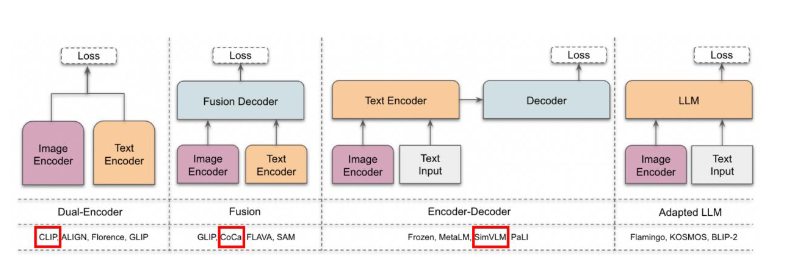
\includegraphics[width=\linewidth]{tikz/chapter11 - CLIP Architectures Recap.png}
    \caption{{\color{red}\colorbox{pink}{Tikz TO-DO}} CLIP Architectures Recap}
\end{figure}

\textbf{Flamingo}, which we will discuss in the next section, blends the dual encoder approach with an \textbf{additional LLM} to further enhance performance.

\section{LLMs as Universal Interface}

Multimodal systems offer a more flexible way to interact with models, allowing the use of different types of input. For example, users can provide input by typing (text), speaking (audio), or using the camera (images or video).

\textit{How can we harness the potential of LLMs to create a general-purpose assistant?} These models need to be able to handle a \textbf{multimodal prompt}, including images and/or video mixed with text. The idea is to equip LLMs with the ability to "see" the world by training them on vision-conditioned language generation tasks. In this way, LLMs can serve as a general interface for other modalities, leveraging the knowledge gained during training on language-only.

\subsection{Frozen LM Prefix}

Now, to better understand Flamingo, we must first introduce the concept of Frozen LM Prefix, described in \href{https://arxiv.org/pdf/2106.13884}{"Multimodal Few-Shot Learning with Frozen Language Models" (Menick et al.)}. 

This model consists of three main components: a \textbf{visual encoder} (NF-ResNet50), a \textbf{language embedder}, and a \textbf{language model for text generation}. The last two components, the language embedder and the language model, are "frozen", meaning that \textbf{their weights are not changed during training or inference}. The resulting textual and visual representations are concatenated and then sent to the language model decoder (LLM), which generates the textual output in an autoregressive manner.

\begin{figure}[!htbp]
    \centering
    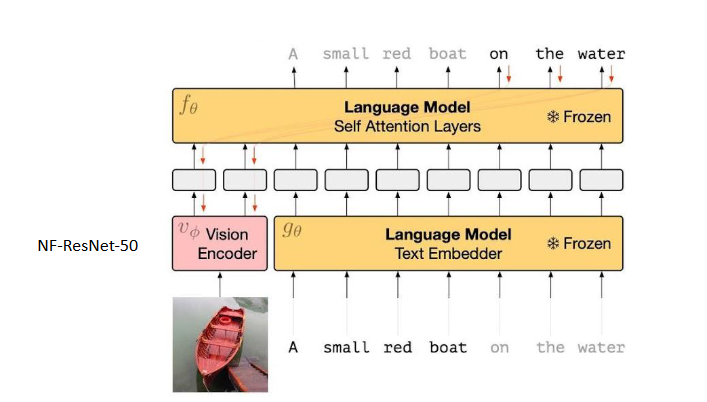
\includegraphics[width=0.8\linewidth]{tikz/chapter11 - Frozen LM.png}
    \caption{{\color{red}\colorbox{pink}{Tikz TO-DO}} Frozen Architecture}
\end{figure}

Subsequently, finetune the image encoder to improve the quality of its representations. Still, its outputs are directly used as soft prompts for the LLM, which means they are used to guide the behavior of the language model without directly modifying its weights. It is like giving a suggestion or a guide to the model on what it should focus on. Here's some examples:

Next, \textbf{fine-tuning of the image encoder is performed} to improve the quality of its representations. However, its outputs are directly used as \textbf{soft prompts} for the LLM, which means they are \textbf{used to guide the behavior of the language model without directly changing its weights}. It is like giving a hint or guidance to the model on what it should focus on. Here are some examples:

\begin{figure}[!htbp]
    \centering
    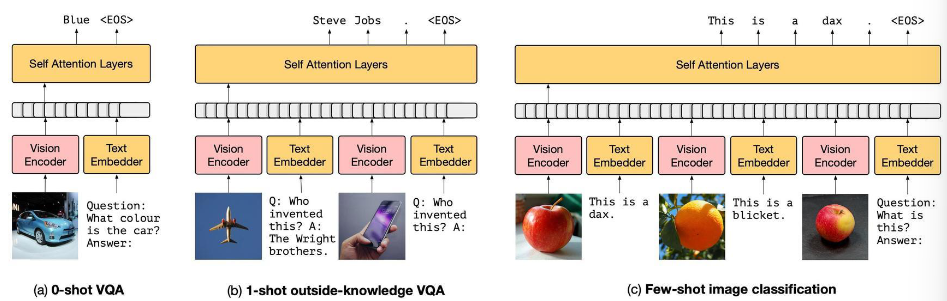
\includegraphics[width=\linewidth]{tikz/chapter11 - Frozen LM Tasks.png}
    \caption{{\color{red}\colorbox{pink}{Tikz TO-DO}} An example of Finetuning Frozen LM}
\end{figure}

\subsection{Flamingo}

Flamingo, developed by Google DeepMind and introduced in \href{https://arxiv.org/pdf/2204.14198}{"Flamingo: a Visual Language Model for Few-Shot Learning" (Donahue et al.)}, represents an advance over previous frozen language models. It links powerful pre-trained visual encoders and pre-trained language models using innovative architectural components.

The model can process images, video, and text, enabling it to perform a variety of tasks such as classification, captioning, question answering, and text completion.

Flamingo's visual encoders, based on a \textbf{Normalizer-Free ResNet architecture}, are trained similarly to CLIP to "perceive" visual scenes. For the textual encoder, Flamingo initially uses \textbf{BERT} instead of GPT-2; however, it is \textbf{discarded after the visual encoder is trained} because it is not used in the final model. Large language models (LLMs) are used to perform basic reasoning tasks.

Flamingo's main innovations include the \textbf{Perceiver Resampler} and \textbf{Gated XATTN-DENSE} layers, which are trained from scratch.

\begin{figure}[!htbp]
    \centering
    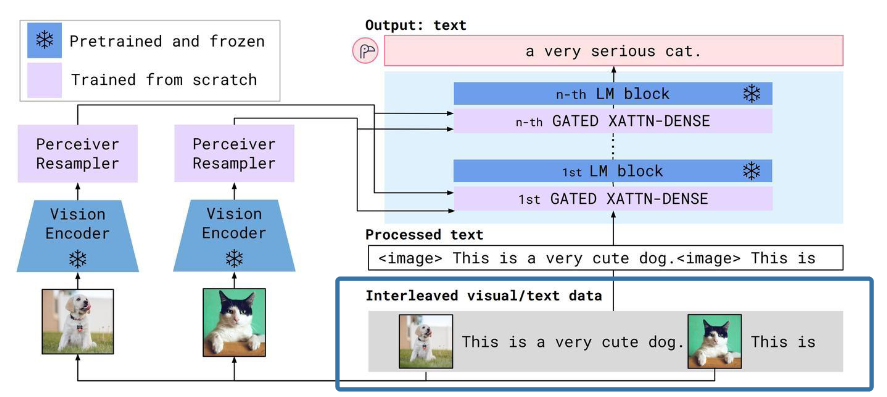
\includegraphics[width=\linewidth]{tikz/chapter11 - Flamingo Architecture.png}
    \caption{{\color{red}\colorbox{pink}{Tikz TO-DO}} Flamingo Architecture}
\end{figure}

The model is trained with sequences of arbitrarily interleaved visual and textual data (\textbf{heterogeneous data}). One challenge of this approach is to \textbf{handle visual inputs of varying sizes}. The Perceiver Resampler addresses this challenge by providing meaningful representations of fixed size. This flexibility allows Flamingo to be trained on \textbf{large-scale multimodal data}.

Flamingo uses \textbf{Chinchilla} as its language model. To generate conditional text on both textual and visual inputs, Flamingo leverages the Perceiver Resampler and Gated XATTN-DENSE layers.





The Perceiver Resampler maps features of variable size to a \textbf{fixed number of output tokens}, regardless of the resolution of the input image or the number of frames in the video. These output tokens, known as latent queries, are a small set learned during training. The output representations from this module are \textbf{later used in the XATT module}.

Gated XATTN-DENSE layers (where XATTN stands for cross-attention) are inserted between the frozen language model layers to \textbf{allow more efficient attention to visual tokens during the generation of textual tokens}. The output of the Gated XATTN-DENSE layers serves as the key, value, and query for the language model layers.

Finally, text is predicted in an autoregressive manner by the language model. 
